\documentclass[12pt,a4paper]{article}
\usepackage[latin1]{inputenc}
\usepackage{amsmath}
\usepackage{amsfonts}
\usepackage{amssymb}
\usepackage{graphicx}
\usepackage{subfig, placeins}
\usepackage[left=1.00in, right=1.00in, top=1.00in, bottom=1.00in]{geometry}
\begin{document}
\noindent Noah Dukler
\section{Methods \& Results}
\subsection{Filtering}
Data for this project were derived from 79 chinese and 107 Yoruban individuals for a total study size of 186 people. The gender breakdown was 92 females and 94 males however only SNP data for chromosome 22 was included for this study so sex specific effects are highly unlikely. SNP data was filtered to remove alleles with MAF$<0.05$ resulting in the removal of 562 variants. The loci were further filtered using a p-value for the Hardy-Weinberg test of $10^{-10}$ to detect any serious genotyping errors resulting in the removal of 216 variants. All individuals were completely genotyped so none were removed. Re-clustering all study individuals based on genotype cleanly recapitulated the ethnic labeling in the HapMap files along the 1st PC with no obvious outliers so no individuals appear to be mislabeled (fig. \ref{fig:mds}). Individuals were not separated by sex along any of the other PCs as expected since the sex chromosomes were not included.   

\begin{figure}[h]
\centering
\includegraphics[width=0.9\linewidth]{../test/cluster_info/mds}
\caption[MDS Plot]{MDS Plot of filtered genotypes. Individuals cleanly separate by ethnicity along PC1 but fail to separate by gender.}
\label{fig:mds}
\end{figure}

The phenotypes of interest were the expression levels of four genes GGT5, MRPL40,TTC38, and FAM118A. The distributions of expression levels were then checked for normality. 

\begin{figure}[h]
\centering
\includegraphics[width=0.9\linewidth, height=7cm]{../test/processed_files/pheno_dist}
\caption[Pheno_dist]{Distribution of expression levels for GGT5, MRPL40, and TTC38 across study population. Data were tested for normality with the Shapiro-Wilk test. Expression data for MPRL and GGT5 were normally distributed with $p>0.05$. Expression levels for TTC38 and FAM118A were non-normally distributed with $p<<0.05$.}
\label{fig:pheno_dist}
\end{figure}

The data for TTC38 and FAM118A were strongly non-normally distributed, violating the assumption of the regression model risking an increased false positive rate so I performed quantile renormalization on all three phenotypes for consistent data treatment \cite{goh_effects_2009}. I also removed individuals NA18573 and NA18637 as their expression levels appeared to be extreme outliers(fig. \ref{fig:pheno_dist}). 

\subsection{Modeling} 
Using PLINK I fit the data to a naive association model of the form:

$$
	Norm.~Gene~Expression = Genotype + \epsilon
$$

\begin{figure}
\includegraphics[width=\linewidth]{../test/norm_basic.plink/plots/merged_qqplot.pdf}
\caption{Histogram and qqplot of p-values derived from fitting basic association model to rank normalized expression data for three genes.}
\label{norm_qq}
\end{figure}   


Genotypes are recoded as $aa=0$, $Aa=1$, and $AA=2$, giving a unique encoding to all allelic combinations. However the p-values resulting from this analysis were left-highly skewed indicating that there would be a high false positive rate resulting from this analysis (fig.\label{norm_qq}). 


This inflation in the frequency of low p-values often results from unmodeled substructure in the population. From our PCA analysis we already know that the study population clusters into two distinct subpopulations based upon ethnicity. Therefore I revise my previous model to include a covariate to model ethnic background as follows: 

$$
	Norm.~Gene~Expression = Genotype + Ethnicity +\epsilon
$$

Ethnicity was recoded by representing CHB individuals as 1 and YRIs as 2. The p-values resulting from fitting this second model were almost uniformly distributed showing that the majority of loci failed to reject the null-hypothesis as expected (aka. were non-causal). Given that the effects of population substructure appear to have been accounted for I proceeded to search for causal loci for the three traits of interest. 

\begin{figure}
\includegraphics[width=\linewidth]{../test/pop_covar.plink/plots/merged_qqplot.pdf}
\caption{Histogram and qqplot of p-values derived from fitting an association model that includes ethnicity to rank normalized expression data for three genes.}
\label{covar_pp}
\end{figure}

\begin{figure}
\label{fig:merged_mhplot}
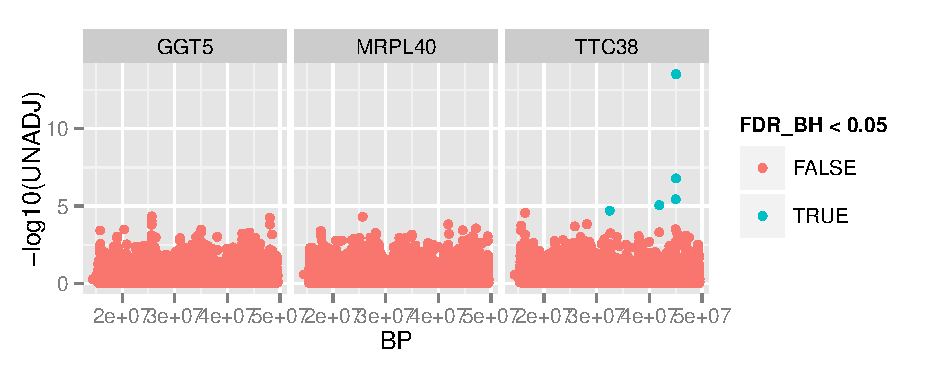
\includegraphics[width=1\linewidth]{../test/pop_covar.plink/plots/merged_mhplot.pdf}
\caption{Manhattan plots of p-values derived from fitting an association model that includes ethnicity to rank normalized expression data for three genes.}
\end{figure}

Of the four genes only two, TTC38 and FAM118A appeared to have any causal eQTLs on chromosome 22 between 14430353 and 49565872bp. Seven potential eQTLs were identified for FAM118A and three identified for TTC38 using an FDR threshold of 0.05 (tab. \ref{eQTL_tab}). The seven SNPS for FAM118A represent 3 LD blocks while the three SNPS for TTC38 represented two (fig \ref{fig:LD}). Thus it appears likely that we have three regions that contain eQTL candidates for FAM118A and two for TTC38.   

\begin{table}
\centering
\begin{tabular}{llrrc}
  \hline
GENE & SNP & BP & FDR\_BH & LD BLOCK\\ 
  \hline
  FAM118A & rs135007 & 41824675 & 2.79e-02 & * \\ 
  FAM118A & rs3827393 & 44114817 & 1.66e-02 & ** \\ 
  FAM118A & rs6006992 & 44121424 & 1.66e-02  & ** \\ 
  FAM118A & rs6007009 & 44160172 & 4.76e-02 & ** \\ 
  FAM118A & rs136604 & 44168407 & 1.66e-02 & ** \\ 
  FAM118A & rs6006743 & 44184187 & 4.76e-02 & ** \\ 
  FAM118A & rs5769966 & 47938808 & 4.76e-02  & *** \\ \hline
  TTC38 & rs6971 & 41888870 & 3.53e-02  & ****  \\ 
  TTC38 & rs6008598 & 45082907 & 3.77e-10  & ***** \\ 
  TTC38 & rs9626816 & 45020262 & 2.16e-02  & ***** \\ 
   \hline
\end{tabular}
\caption[eQTL]{Causal eQTLs identified by model that included an ethnic covariate.}
\label{eQTL_tab}
\end{table}

\begin{figure}
\centering
\subfloat[LD for FAM118A\label{fig3:test1}]
  {\includegraphics[width=.5\linewidth]{../test/LD/plots/FAM118A_LD}}\hfill
\subfloat[LD for TTC38 \label{fig3:test2}]
  {\includegraphics[width=.5\linewidth]{../test/LD/plots/TTC38_LD}}\hfill
\caption{Clustered LD profiles for TTC38 candidate eQTLs.}
\label{fig:LD}
\end{figure}

\section{Discussion}
\subsection{FAM118A}
\begin{figure}
\centering
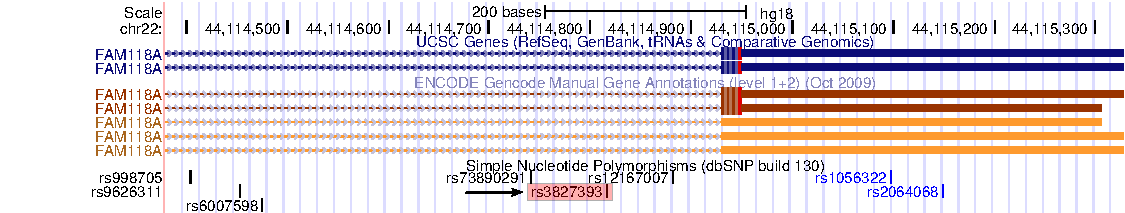
\includegraphics[width=1\linewidth]{./hgt_genome_28d3_4cda30}
\caption{UCSC genome browser shot of rs3827393.}
\label{fig:hgt_genome_28d3_4cda30}
\end{figure}


	FAM118A is a protein coding gene roughly 32Kb long however its function is unknown. It is highly unlikely rs135007 is an eQTL as it is roughly 2.2 Mb upstream of FAM118A, outside the observed range for a cis-eQTL. Furthermore is an intron variant and thus unlikely to affect the functional form of the gene that it is in, reducing the likelihood of it being a trans-eQTL. Of the cluster of 5 SNPs in LD the one most likely to be a causal variant is rs3827393 as it is within an intron of FAM118A itself (fig. \ref{fig:hgt_genome_28d3_4cda30}). It is common to see regulatory elements in the introns of the genes they regulate but with out ChIP-seq for histone marks in the appropriate cell line it is impossible to guess at functional mechanism. The SNP is the third LD block, rs5769966, is unlikely to be causal as it is almost 4Mb downstream of FAM118A (unlikely to be a cis-eQTL) and it is not a coding variant (unlikely to be a trans-eQTL).     

\subsection{TTC38}
     TTC38 (tetratricopeptide repeat domain 38) is a protein-coding gene whose function has not yet been elucidated. One of the candidate eQTL is rs6971 which is in an exon of the TSPO gene. Rs6971 is a missense coding variant that renders the gene non-functional. TPSO is a translocator protein which moves cholesterol into the mitochondria as part of steroid hormone synthesis. While rs6971 is almost certainly important in TPSO function and has been previously linked to bipolar disorder there is no evidence of a protein-protein interaction between TPSO and TTC38 \cite{colasanti_bipolar_2013}. However TTC38 does interact with RDH13, a retinol dehydrogenase which may help protect the mitochondria against oxidative stress \cite{franceschini_string_2013}. Thus TTC38 and TPSO are linked in a roundabout way however given that rs6971 is in a coding region, has other clear functional activity, and showed a relatively weak association with TTC38 expression, it is unlikely to be causal. Perhaps the association is simply correlative, when one part of the steroid synthesis fails, the expression other genes that are involved (potentially) change as well.
     
     The most likely region for the causal SNP is marked by two SNPs, rs6008598 and rs9626816 which are in LD. Of those three rs6008598 has the most significant association by a significant margin. However rs6008598 is located in the coding region of the GTSE1 protein and it is a synonymous mutation thus making it unlikely that it is the causal mutation itself. Instead it is probably some other SNP in LD with rs6008598. The other SNP in LD is rs9626816, is in an intron of C22ORF40. The intron is only 20kb upstream of TTC38 which is well withing the range of a normal enhancer element. ChIP-seq for H3K3me3, or CAGE, or PRO-seq within the cell line that the HapMap data I analyzed would be necessary to provide further evidence for rs9626816 being part of an enhancer sequence.                 

\FloatBarrier

\bibliographystyle{nature}
\bibliography{GWAS}

\end{document}